%%	SECCION documentclass																									 %%	
%%---------------------------------------------------------------------------%%
\documentclass[a4paper]{report}

%%---------------------------------------------------------------------------%%
%%	SECCION usepackage																											 %%	
%%---------------------------------------------------------------------------%%
\usepackage{amsmath, amsthm}
\usepackage[spanish,activeacute]{babel}
\usepackage{caratula}
\usepackage{a4wide}
\usepackage{hyperref}
\usepackage{fancyhdr}
% \usepackage{moreverb}
\usepackage{graphicx} % Para el logo magico!
\usepackage{capt-of}
\usepackage{afterpage}
\usepackage{float}
\usepackage{amssymb}
\usepackage{amsmath}
\usepackage[latin1]{inputenc}
\usepackage{subfigure}
\usepackage[dvipsnames,usenames]{color}
\usepackage{amsfonts}
\usepackage{pdflscape}
\usepackage{booktabs}
\usepackage{colortbl}
\usepackage{tabularx}
\usepackage{ifthen}

%%---------------------------------------------------------------------------%%
%%	SECCION opciones																												 %%	
%%---------------------------------------------------------------------------%%
\parskip    = 11 pt
\headheight	= 13.1pt
\pagestyle	{fancy}
\definecolor{orange}{rgb}{1,0.5,0}

\addtolength{\headwidth}{1.0in}

\addtolength{\oddsidemargin}{-0.5in}
\addtolength{\textwidth}{1.0in}
\addtolength{\topmargin}{-0.5in}
\addtolength{\textheight}{0.7in}

%%---------------------------------------------------------------------------%%
%%	SECCION document	 %%	
%%---------------------------------------------------------------------------%%
\begin{document}
\renewcommand{\chaptername}{Parte }

%%---- Caratula -------------------------------------------------------------%%
\materia{Ingenier�a de Software I (2do cuatrimestre de 2008)}
\titulo{Trabajo Pr�ctico 1}

\integrante{Gonzalez, Emiliano}{426/06}{xjesse\_jamesx@hotmail.com}
\integrante{Gonzalez, Sergio}{481/06}{seges.ar@gmail.com}
\integrante{Mart'inez, Federico}{17/06}{federicoemartinez@gmail.com}
\integrante{Sainz-Tr�paga, Gonzalo}{454/06}{gonzalo@sainztrapaga.com.ar}
\grupo{Grupo 5}
\resumen{
Se presenta en este trabajo una especificaci�n completa de la soluci�n propuesta para el proyecto de software de
administraci�n de pizzer�a. En el mismo se presenta un panorama general as� como un an�lisis detallado del problema, 
y nuestra propuesta para su resoluci�n. En primer lugar se plantea una descripci�n general de la soluci�n, y a
continuaci�n se detallan algunos aspectos importantes haciendo uso de herramientas desarrolladas en clase como
diagramas de actividad, m�quinas de estado finito y otras.
}

\definecolor{light-gray}{gray}{0.9}

\newcommand{\clase}[4]{
\subsection{#1}
#2
\ifthenelse{\equal{#3}{}}{}
{\subsubsection{M�todos}
#3
} 
\ifthenelse{\equal{#4}{}}{}
{
\subsubsection{Atributos}
#4
}
}

% ----- Token list para las instrucciones ------------------------------------
\newtoks\oplist\oplist={}
% ----- Comando para que el usuario agregue operaciones del CU

\newcounter{PasoCu}
\setcounter{PasoCu}{1}

\newcommand{\op}[2]
{
\oplist=\expandafter{\the\oplist #1 & #2 \\ \hline}
\stepcounter{PasoCu}
}
\newcommand{\negrita}[1]{{\bf #1}}
\newcounter{casoUso}
\setcounter{casoUso}{1}

\definecolor{light-gray}{gray}{0.9}
\newcommand{\cu}[6]{ 
{\setlength{\arrayrulewidth}{1mm}

\begin{tabularx}{16cm}{|X|X|}
\hline
\multicolumn{2}{|>{\columncolor{Black}}l|}{\textcolor{White}{\negrita{Caso de Uso: #1}}} \\
\hline
\multicolumn{2}{|>{\columncolor{Black}}l|}{\textcolor{White}{\negrita{N�mero \thecasoUso}}} \\
\hline
\multicolumn{2}{|>{\columncolor{light-gray}}l|}{\negrita{Actores intervinientes: #2}} \\
\hline
\multicolumn{2}{|>{\columncolor{light-gray}}l|}{\negrita{Requerimientos relacionados: #3}} \\
\hline
\multicolumn{2}{|>{\columncolor{light-gray}}l|}{\negrita{Precondici�n: #4}} \\
\hline
\multicolumn{2}{|>{\columncolor{light-gray}}l|}{\negrita{Poscondici�n: #5}} \\
\hline
\multicolumn{1}{|>{\columncolor{light-gray}}X|}{\negrita{Descripcion:}} &
\multicolumn{1}{>{\columncolor{light-gray}}X|}{\negrita{#6}} \\
\hline
\multicolumn{1}{|>{\columncolor{light-gray}}X|}{\negrita{Curso normal}} &
\multicolumn{1}{>{\columncolor{light-gray}}X|}{\negrita{Curso alternativo}}\\
\hline
\the\oplist
\end{tabularx}
\stepcounter{casoUso}
}
\newtoks\oplist\oplist={}
}

% TOC, usa estilos locos
\maketitle
\pagestyle{empty}
{
\fancypagestyle{plain}
    {
    \fancyhead{}
    \fancyfoot{}
    \renewcommand{\headrulewidth}{0.0pt}
    } % clear header and footer of plain page because of ToC
\tableofcontents
}

\newpage
% arreglos los estilos para el resto del documento, y
% reseteo los numeros de pagina para que queden bien
\pagenumbering{arabic}
\fancypagestyle{plain} {
    \fancyhead[LO]{Gonzalez, Gonzalez, Mart�nez, Sainz-Tr�paga}
    \fancyhead[C]{}
    \fancyhead[RO]{P\'agina \thepage\ de \pageref{LastPage}}
    \fancyfoot{}
    \renewcommand{\headrulewidth}{0.4pt}
}
\pagestyle{plain}

\chapter{Modificaciones a la especificaci�n}

Al momento de realizar el dise�o, decidimos realizar ciertas modificaciones a la 
especificaci�n presentada en el informe anterior. A continuaci�n, explicaremos cu�les 
fueron estas modificaciones, cu�l fue la motivaci�n para realizarlas y qu� impacto tienen
en el sistema resultante.

\section{Identificaci�n individual de los m�dulos del horno}

Se decidi� llevar a cabo una modificaci�n que anteriormente hab�a sido considerada
una mejora a futuro: los m�dulos de los hornos ser�n identificables de forma �nica,
mientras que antes se los consideraba indistinguibles.

\subsection{Justificaci�n}
Ya en el trabajo anterior establecimos que no identificar los m�dulos del horno
conlleva un problema de usabilidad, ya que cuando un cocinero extrae comidas del horno
no puede indicarle al sistema r�pidamente que fue lo que sac�, sino que debe
indicar qu� productos estaban en ese m�dulo y el sistema deber� entonces reconocer qu�
pedido sali� del horno.

En esta situaci�n, si dos m�dulos tienen los mismos
items, hay que recurrir a una decisi�n heur�stica para determinar qu�
m�dulo corresponde a cada pedido (como por ejemplo, ``el que entr�
primero va a al pedido que ingres� antes''), pero esto podr�a resultar
en que los productos cocinados se asignen incorrectamente a los
pedidos cuando salen del horno, y esto hace que no funcione como se
espera la pol�tica de cola.

Por otra parte, si bien en pol�tica de cola normal no es indispensable
realizar la distinci�n, s� lo es en el caso de la pol�tica �gil de cola. Como
decidimos separar la pol�tica del mecanismo utilizado para llevarla a cabo,
resultaba razonable ofrecer a toda pol�tica de horno los medios necesarios
para funcionar. Esto involucrar�a una diferencia muy grande de funcionamiento
entre la pol�tica de cola normal y la pol�tica de cola �gil. Esto redunda
en c�digo m�s complejo y acoplado. Por otra parte, la identificaci�n
individual de los m�dulos representa un servicio minimalista y que es
razonable para muchas pol�ticas distintas que pudieran implementarse. En
funci�n de eso, consideramos que es mucho m�s extensible esta modalidad.

En particular, si no se desea distinguir m�dulos entre ellos, es necesario
en la pol�tica �gil distinguir dos ``categor�as'' de los mismos: �giles y
normales. La distinci�n individual de m�dulos permite al sistema hacer todo
tipo de categorizaci�n, y el cocinero solo debe indicar de qu� m�dulo se
trata (y no caracter�sticas \textit{ad hoc} a la pol�tica tales como si
el m�dulo es �gil o no).

\subsection{Impacto del cambio}
En esta secci�n realizaremos una revisi�n de que cambios acarrea a la 
operatoria la identificaci�n individual de los m�dulos.

A nivel de objetivos este cambio nos agrega un requerimiento nuevo, que 
consiste en mantener la informaci�n de los m�dulos. La figura \ref{objetivos} 
permite observar el fragmento del diagrama que se ve modificado por el cambio.

\begin{figure}[H]
\centering
\subfigure[Diagrama de objetivos original]{
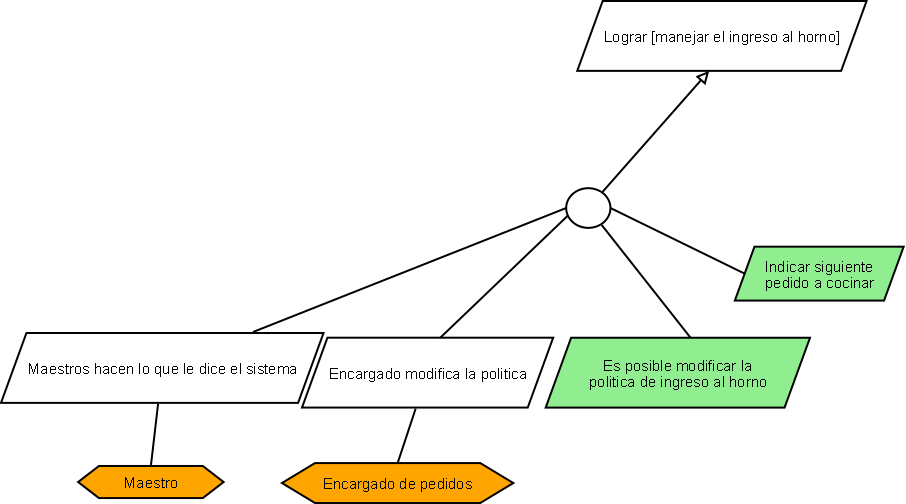
\includegraphics[scale=0.3]{./figuras/objetivos_viejos.png} }
\subfigure[Diagrama de objetivos modificado]{
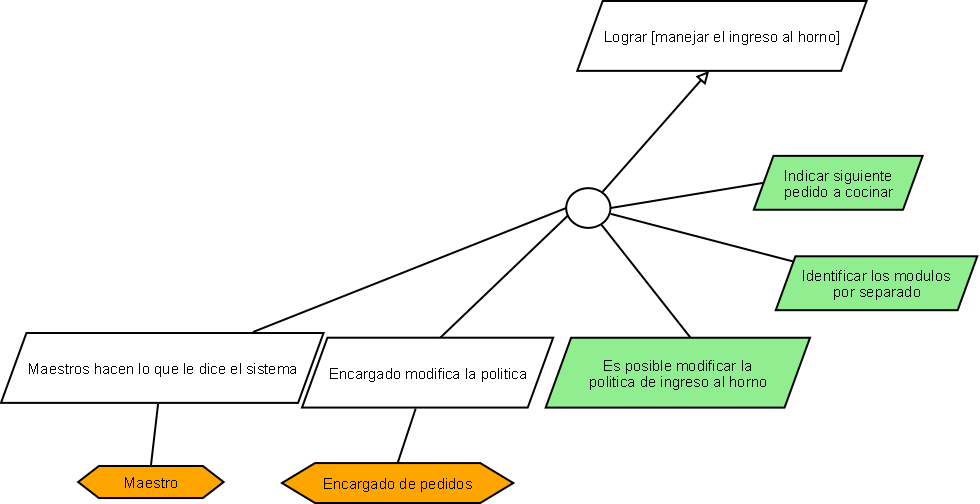
\includegraphics[scale=0.3]{./figuras/objetivos_nuevo.png}}
\label{objetivos}
\caption{Impacto en el modelo de objetivos}
\setcounter{subfigure}{0}
\end{figure}

A nivel del diagrama de contexto no se producen cambios produce un cambio mayor,
ya que las comunicaciones entre agentes se mantienen (si bien la informaci�n transmitida
es levemente distinta cuando el maestro de cocina se comunica con el sistema). En cambio, s� 
se genera un cambio en la descripci�n de los casos de uso relacionados con la cocci�n de los
productos. En particular, se modifican los casos de uso \textit{Indicando producto cocinado} y
\textit{Siendo informado de pr�ximo pedido a cocinar}. Se detalla a continuaci�n.

% Indicando producto cocinado
\op{1. El maestro indica al sistema que finaliz'o la cocci'on de ciertas partes de un pedido, seleccionando el m�dulo que desaloja}{}
\op{2. El sistema registra la parte como cocinada}{}
\op{3. El sistema verifica si la 'ultima parte cocinada completa el pedido}{}
\op{4. Si es as'i, el sistema registra al pedido como listo}{}
\op{5. Si hay productos para cocinar el sistema le informa al maestro que de debe poner a continuaci�n. EXTIENDE caso de uso Siendo informado de proximo producto a cocinar}{}
\op{6. Fin CU}{}
\cu{Indicando producto cocinado}{Maestro}{8, 11, 12, 15, 33}{True}{La parte de pedido se registra como cocinada}{El maestro, luego de cocinar una parte de un pedido, indica al sistema que la misma est'a cocinada}

% Siendo informado de proximo pedido a cocinar
\op{1. El sistema indica al maestro una parte a cocinar y qu� m�dulo libre le corresponde}{}
\op{2. Si es la primera parte de un pedido, el sistema cambia el estado del mismo a ``En Horno''}{}
\op{4. Fin CU}{}
\cu{Siendo informado de pr�ximo producto a cocinar}{Maestro}{8, 11, 12, 15, 33}{La cola del horno no est'a vac'ia}{La parte comienza a cocinarse}{El sistema le ordena al maestro que parte de pedido debe cocinar y en que m�dulo del horno}

Con respecto al funcionamiento del ingreso al horno, este es similar al funcionamiento anterior, 
pero ahora el maestro deber� indicar qu� modulo libera, y el mismo sistema se encargar� de deterinar
si el mismo era �gil o no. Esto es m�s razonable ya que dicha decisi�n puede ser realizada por
la pol�tica de cola, que es la entidad m�s id�nea para hacerlo.

%TODO: hacer 2 diagramas de actividad, uno cuando se libera modulo agil y otro cuando se libera un modulo no agil

\section{Estimaci�n de tiempos}
\label{modifEstim}

Se modific� el algoritmo de estimaci�n de tiempos de preparaci�n y cocci�n de pedidos
por uno m�s fiable, ya que se encontraron errores en el algoritmo propuesto en la
especificaci�n.

\subsection{Justificaci�n}
En la especificaci�n presentamos una operaci�n para realizar la estimaci�n que, si 
bien permit�a obtener una cota superior al tiempo necesario para terminar un pedido, resultaba
en muchos casos una estimaci�n muy grosera. En particular, el algoritmo consideraba al
horno como un proceso secuencial, mientras que �ste tiene la capacidad de cocinar muchos
productos en paralelo. Si bien la estimaci�n anterior da un alto grado de confianza en que
no se exceda el tiempo estimado, subestima muy fuertemente la capacidad de producci�n en la
cocina y en momentos de mucha ocupaci�n la cota superior puede tomar valores rid�culos.

Consideremos un ejemplo: La pizzer�a no tiene pedidos, y se realiza un pedido de 6 pizzas, 
donde cada pizza tarda 30 minutos en cocinarse y consideremos despreciable el tiempo de preparaci�n.
Supongamos tambi�n que en el horno entran 6 pizzas al mismo tiempo. En este caso una buena estimaci�n 
ser�a 30 minutos. Sin embargo, por como calculabamos la estimaci�n, la misma ser�a de 3 horas, lo
cual es excesivo al punto que es probable que el cliente cancele el pedido.

%FIXME: fede hijo de puta hablas como el chavo
% Dec�a: "3 horas, lo cual es un tiempo mucho muy grande"

Por esta raz�n decidimos utilizar una nueva m�trica para calcular el tiempo estimado. La idea no 
es dar un tiempo exacto, sino corregir la sobreestimaci�n grosera que generaba la operaci�n anterior.
La nueva operaci�n de estimaci�n es la siguiente:

$$tiempoEstimado(p) = tiempoPreparacion(p) + \sum{tiempoPreparacion(ped)} + $$
$$ \frac{tiempoCoccionPizzasDe(p)+ \sum{tiempoCoccionPizzasDe(peds)}}{pizzasPorModulo*modulosPorHorno} + $$ 
$$ \frac{tiempoCoccionEmpanadasDe(p) + \sum{tiempoCoccionEmpanadasDe(peds)}}{EmpanadasPorModulo*modulosPorHorno}$$

donde $ped$ son los pedidos que est�n por ingresar o esperando prepararse, y $peds$ son los pedidos que est�n 
esperando por ingresar a cocina, prepararse o ingresar al mismo horno asignado a $p$.

Si bien el dise�o que presentamos a continuaci�n permite reemplazar f�cilmente el algoritmo
de estimaci�n de tiempos por otros m�s sofisticados y precisos, consideramos necesario corregir
este error para proveer al cliente de una opci�n razonable desde la entrada en producci�n del
sistema.

\subsection{Impacto del cambio}
Dado que la estimaci�n de tiempos es una operaci�n interna de la que lo �nico que observa
el usuario es el resultado, no involucra modificaciones en la especificaci�n del sistema.

\chapter{Clases}
\section{Modelado de clases}
Nuestra primer idea al modelar la soluci�n, fue identificar los diversos componentes logicos presentes en el sistema. De esta manera pudimos identificar la existencia de grupos de funcionalidades que se pod�an agrupar. Consideramos la existencia de los siguientes componentes:

\begin{figure}[H]
\centering
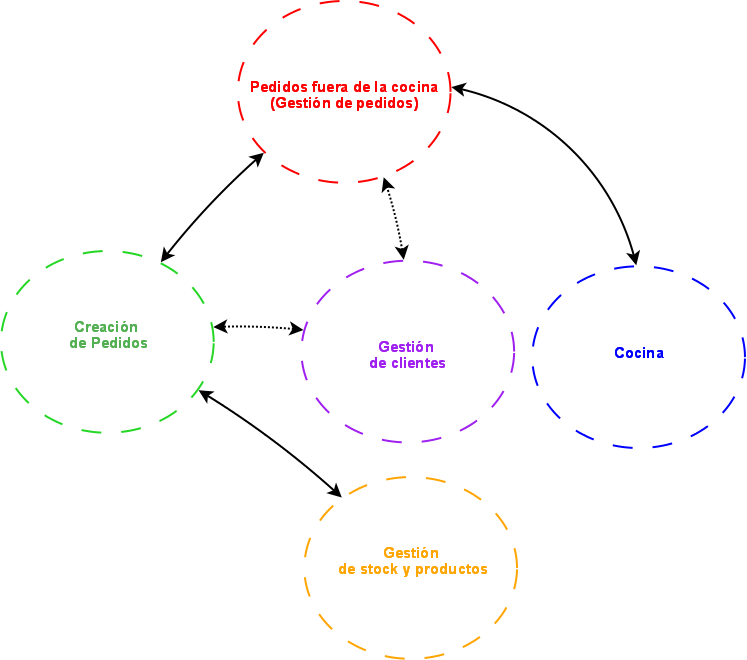
\includegraphics[height=10cm]{./figuras/divisionModelo.png}
\caption{Esquema de componentes l�gicos}
\end{figure}
%FIXME: el dibujo mepa q esta mal
\begin{itemize}
\item Pedidos fuera de la cocina: Este componente agrupa las funcionalidades del ingreso, despacho, consulta de estado y otros aspectos que involucren a las partes del ciclo de vida que no ocurran en el ambito de la cocina.
\item Creaci�n de pedidos: Aqu� se agrupan aquellas funcionalidades que hacen posible que se creen e ingresen al sistema nuevos pedidos. Podr�a considerarse parte de Pedidos fuera de la cocina, pero sin embargo la creaci�n tiene una logica bastante compleja de estimaci�n de tiempos, chequeo de stock, entre otras cosas que nos llevaron a considerarlo como un componente separado.
\item Gesti�n de clientes: Este componente permite realizar las validaciones de clientes asi como tambi�n las altas, bajas y modificaciones de clientes
\item Cocina: Aqui se engloban las funciones que permiten guiar la preparaci�n y cocci�n de un pedido.
\item Gesti�n de stock y productos: En este componente se engloba el ABM de stock y el ABM de productos
\end{itemize}

Esta divisi�n sirve para gu�a pero no es estrictamente asi, ya que por ejemplo la cancelaci�n es un evento que toca tanto a la cocina como a los pedidos fuera de esta, por otro lado el Pedido como tipo de datos es utilizado por todos los componentes en mayor o menor medida. No obstante creemos que esta divisi�n en componentes sirve para mostrar el enfoque que se le dio al dise�o

\section{Pedidos fuera de la cocina}
Como dijimos este componente tiene por responsabilidad el manejo de la vida de los pedidos que estan fuera de la cocina (por cocina entendemos no solo al horno, sino tambi�n a la preparaci�n de los pedidos).

Nuestra idea fue tener un coordinadorDePedidos que siga el patron Fa�ade, de modo que muestre a la interfaz grafica una intrefaz \textit{``gruesa''} con las funciones que se realizan dentro del componente. Esta clase no va a tener gran inteligencia, sino que se limitara a propagar la llamada originada por la interfaz grafica a la clase responsable de manejar esa llamada. As�, por ejemplo para ver el estado de un pedido o ingrear un nuevo pedido se deber� pasar por esta clase.
La idea de esta clase es desacoplar la interfaz grafica de las clases que manejan a los pedidos fuera de la cocina. Si bien esta clase para tener baja cohesi�n, al mirarla de cerca vemos que lo �nico que hace es derivar las llamadas. De este modo si bien a trazo grueso parece tener una interfaz con poca cohesi�n, esta nos permite lograr un menor grado de acoplamiento entre la interfaz y el sistema en si. Por esta raz�n decidimos pese al aparente conflicto con la cohesi�n, decidimos mantener esta clase.
Ademas el coordinadorDePedidos se comunica con el componente encargado de crearPedidos, haciendo de puente entre ambos componentes.
Cuando se realiza un pedido de ingreso, el coordinador se encarga de pedir que se genere el pedido, y en caso de que se pueda crear, lo deriva al controladorDePreIngreso, cuya funci�n es determinar si el pedido debe ir a la cola de listos, porque no hay nada que preparar, ni cocinar, o lo tiene que mandar al controlador de ingreso, porque hay algo que cocinar o preparar. Este comportamiento se hizo con la intenci�n de permitir en un futuro incorporar otros productos ademas de pizzas o empanadas. Por ejemplo, podrian venderse ensaladas, las cuales no requieren de cocci�n, pero si de preparaci�n. Por eso decidimos que un producto tuviera atributos de cocinable y preparable.

El controladorDeIngreso se encarga de mantener la cola de ingreso, asi como de suministrar los pedidos al CoordinadorDeCocina, para que este los distribuya al preparador o al coordinador de horno.
El coordinadorDeIngreso puede recibir recibir una solicitud de un pedido de cierto tipo por parte del CoordinadorDeCocina, por ejemplo puede recibir una solicitud del proximo pedido que contenga algun producto del tipo empanada. 
Por otro lado, cada vez que ingresa un nuevo pedido, el controladorDeIngreso pregunta al CoordinadorDeCocina si puede recibir dicho pedido. Esta funcionalidad sirve para aquellos casos en los que por ejemplo no hay ningun pedido ingresado con empanadas y el maestro empanadero esta ocioso. Si llega un nuevo pedido con empanadas, el maestro debe ser notificado, por esta razon el ControladorDeIngreso pregunta si debe encolar el pedido o hay alguien que lo vaya a preparar.
%FIXME: la parte de preguntar es propia del standard, es decir del concreto

Otra clase de este componente, es el ControladorDeListos, este controlador va a recibir los pedido listos y va a encargarse en el momento del despacho de decidir que hacer con el pedido. Por ejemplo si es un pedido con delivery hay que marcar que salio con el delivery, y si era local hay que marcarlo como finalizado.

La clase controladorDeEntragas contiene a todos los pedidos cuya entrega esta pendiente, y se encargan de finalizar el pedido cuando se notifica la entrega.

Por ultimo el controladorPedidosMesa monitorea los pedidos entregados a una cierta mesa, permitiendo que al cerrar la mesa se fijen sus formas de pago.

La clase controladorDeIngreso es abstracta porque consideramos que la estrategia con la que se maneja la cola de ingreso podria cambiar, de esta manera la versi�n propuesta por nosotros en la etapa de especificaci�n es implementada por controladorDeIngresoStandard. Utilzar una clase abstracta nos permite lograr flexibilidad si se quiere cambiar de politica de manejo de esta cola, por ejemplo usando un manejo del tipo mas corto primero.


\textcolor{Red}{TODO: interacciones de estas clases con la GUI}

\textcolor{Red}{TODO: explicacion de metodos importantes}

\subsection{Modelado de escenarios}
%FIXME: en el ingreso se da a la gui la responsabilidad de mostrar los datos del pedido, tiempo estimado y precio, no se si eso esta bien
\subsubsection{Ingreso de un pedido de solo bebidas}
A continuaci�n intentaremos mostrar las interacciones existentes en este componente con el fin de modelar su comportamiento.
Como primer escenario veamos que ocurre cuando ingresa un pedido de solo bebidas Telefonico. En este caso el pedido ser� creado por el generador de pedidos, sin embargo las interacciones propias de la creaci�n no se detallaran en este escenario, asi como tampoco la validaci�n previa del cliente. Una vez que el pedido es creado, pasa al controlador de pre ingreso que lo examina para decidir si debe ir a la cocina o considerarse un pedido listo. En este caso, como solo hay bebidas, el pedido queda listo. El controlador de listos agrega el pedido a su lista de pedidos, se hace responsable del mismo y cambia su estado. 
Al agregar el pedido a la lista notifica a su observador de que ocurrio un cambio, por ejemplo para que se repinte la lista de pedidos listos.

\begin{figure}[H]
\centering
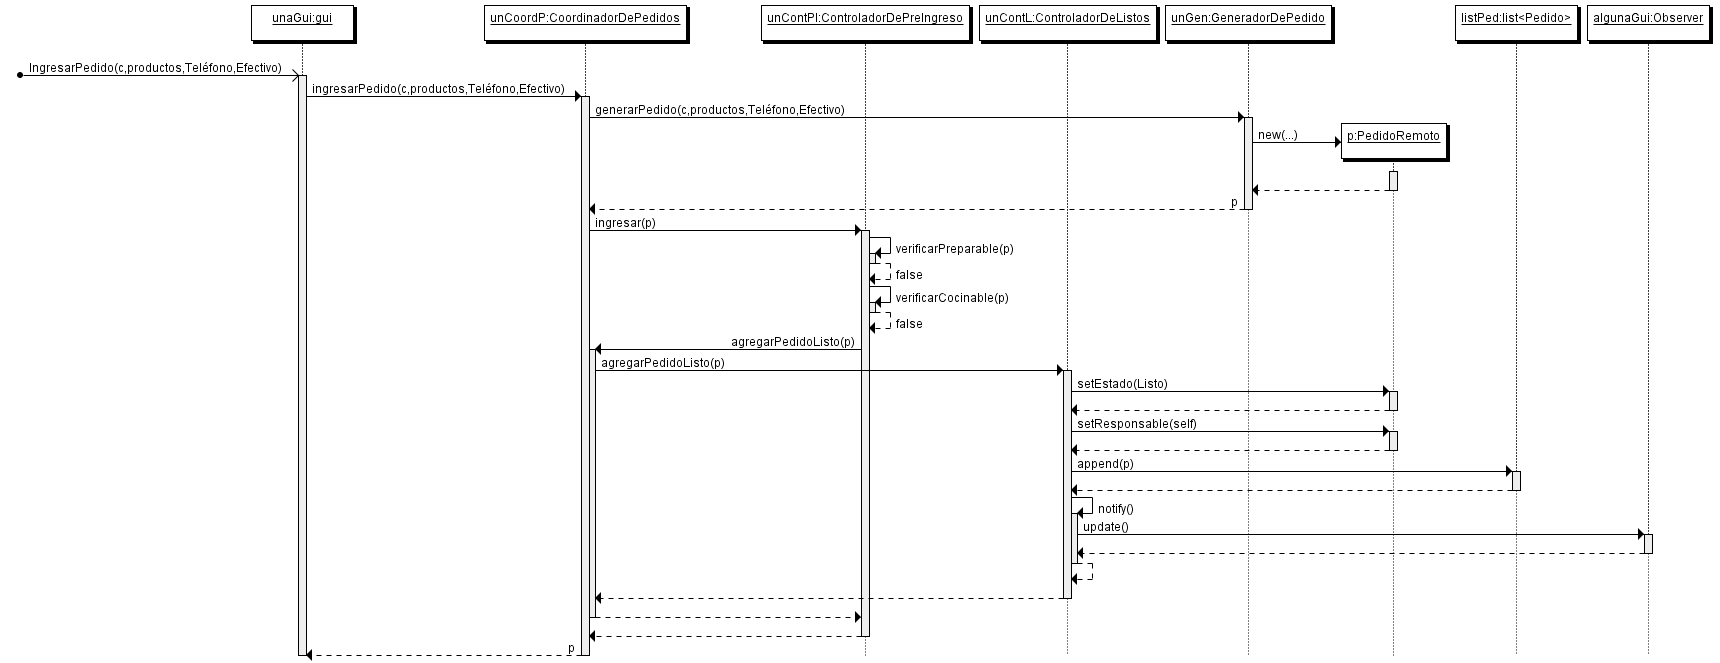
\includegraphics[height=9cm]{./figuras/remotoBebidas.png}
\caption{Ingreso de un pedido remoto de solo bebidas}
\end{figure}

El verifcarPreprable y su analogo para cocinable, basicamente recorren los productos del pedido, buscando si alguno tiene un tipo preparable o cocinable.

\begin{figure}[H]
\centering
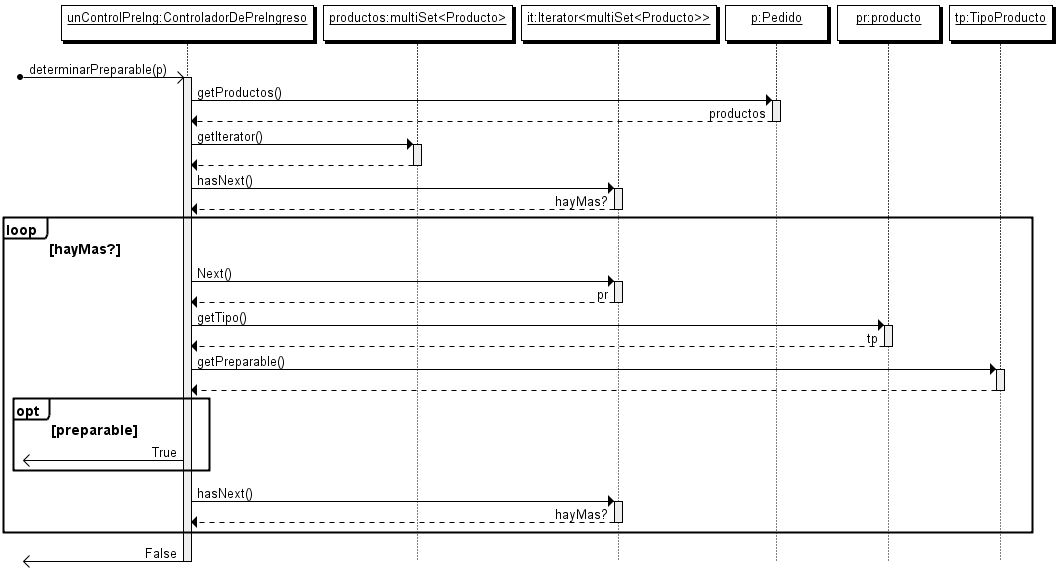
\includegraphics[height=9cm]{./figuras/determinarPreparable.png}
\caption{VerificarPreparable}
\end{figure}

\begin{figure}[H]
\centering
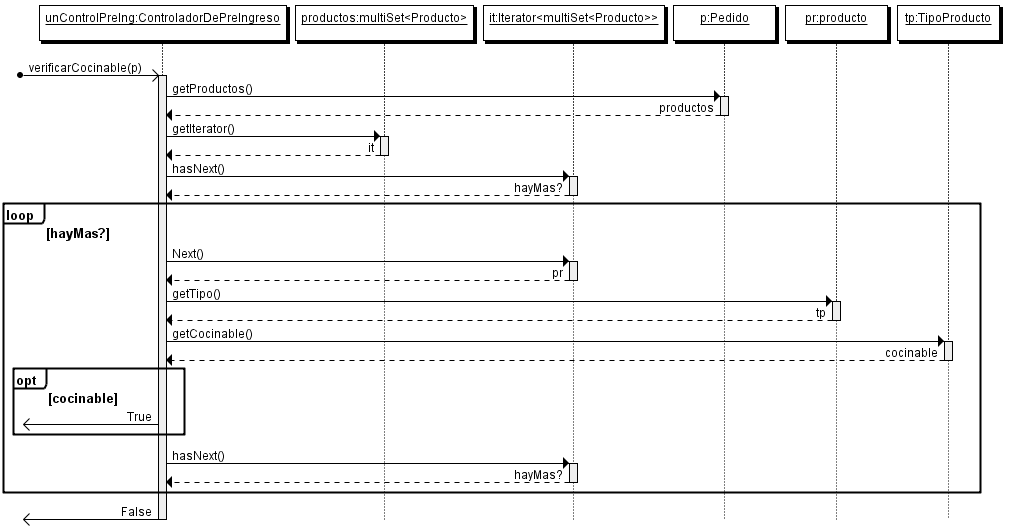
\includegraphics[height=9cm]{./figuras/determinarCocinable.png}
\caption{VerificarCocinable}
\end{figure}
%FIXME: o tocamos la imagen con el inkscape o justifamos las cosas que son de notacion rara

\subsubsection{Ingreso de un pedido con comidas}
De forma analoga al escenario anterior, supongamos que se va a ingresar un pedido, pero en este caso, el pedido si ten�a comidas, por lo que el controlador de pre ingresos se lo va a mandar al de ingresos. Este intenta pasarlo a la cocina para ver si esta puede hacerse cargo del pedido. Esto es asi porque en la especificaci�n se pide que si entra un pedido y el maestro estaba ocioso, se le notifique que prepare el pedido ingresado. Como conocer si los maestros estan preparando algo, no es asunto de este controlador lo que decidimos es que lo pase hacia la cocina y espere respuesta de esta. Modelaremos los dos escenarios, primero el caso en el que la cocina le dice que no puede hacerse cargo y en segundo lugar el caso en el que la cocina si acepta el pedido.

En el primer caso, el controlador de ingresos se hace cargo del pedido, cambiando su estado, marcando el pedido como ingresado y agregandolo a la cola.

\begin{figure}[H]
\centering
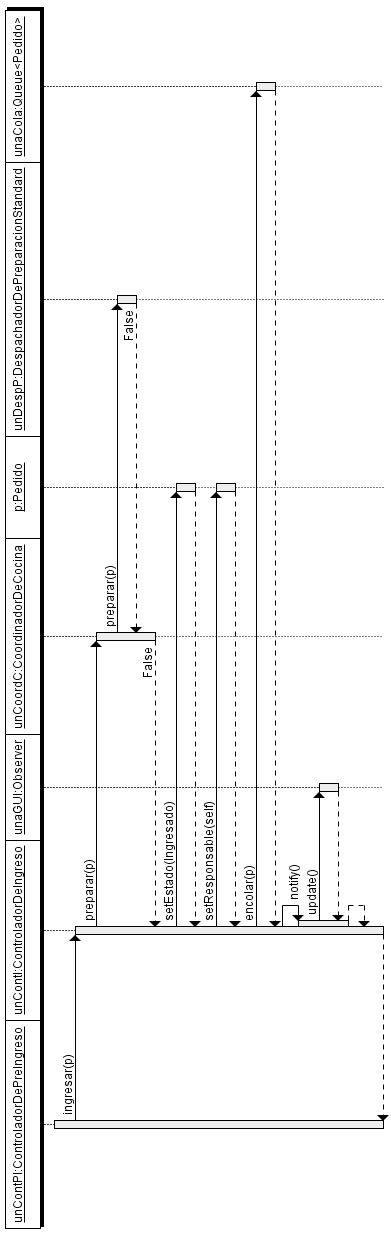
\includegraphics[height=7cm]{./figuras/remotoComidas.png}
\caption{Ingreso de un pedido remoto con comida que queda encolado para su ingreso}
\end{figure}

En el segundo caso, como se va a hacer cargo la cocina, el controlador de ingreso no debe hacer nada cuando se regresa la llamada.

\begin{figure}[H]
\centering
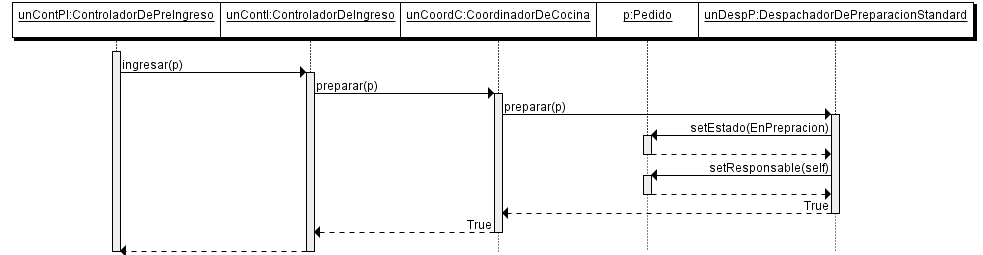
\includegraphics[height=5cm]{./figuras/remotoComidasquedapreparando.png}
\caption{Ingreso de un pedido remoto con comida que pasa a estar preparando}
\end{figure}

\subsubsection{Despacho de un pedido}
Cuando el pedido esta cocinado es responsabilidad de el controlador de listos. Una vez que el pedido esta listo, se puede despachar. Despachar tiene una semantica diferente segun el origen del pedido, por eso es que el controlador posse un despachar para los subtipos remotos, otro para el pedido de mesa y finalmente un tercer despachar para pedidos de mostrador.

En el escenario en el cual el pedido a despachar es de origen remoto, el controlador de listos, lo que hace es sacarlo de la lista, marcarlo como que salio en entrega y avisar de esto al coordinadorDePedido para que avise al controlador de entrega. Ademas notifica a su observador del evento. Esto se hace con la intenci�n de que la gui se entere de que un pedido salio de esta lista y la refresque.

El controlador de entregas pone al pedido en su lista de pedidos, y se asigna como responsable de la cancelaci�n del mismo.

Veamos el diagrama de secuencia comenzando la misma con la llegada de un mensaje de despachar al coordinador de pedidos

\begin{figure}[H]
\centering
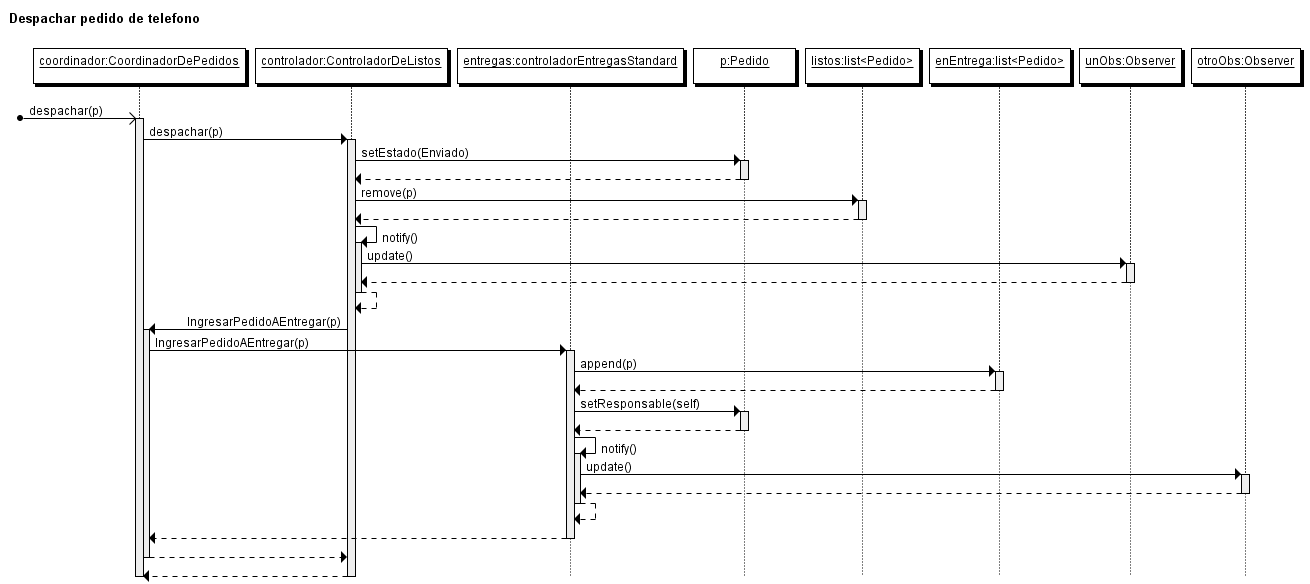
\includegraphics[height=5cm]{./figuras/despacharPedidoTelefono.png}
\caption{Despacho de un pedido telefonico}
\end{figure}

Otro escenario diferente lo constituye el despacho de un pedido de mesa. En este caso, el pedido deja la orbita del controlador de lista, para pasar al controlador de pedidos de mesa, el cual se encargara cuando se cierre la misma de asignar la forma de pago a los pedidos. Este encargado tambi�n se hace cargo de la cancelaci�n. Ambos controladores ademas notifican a su observador de los cambios en su lista.

El diagrama de secuencia es el siguiente:

\begin{figure}[H]
\centering
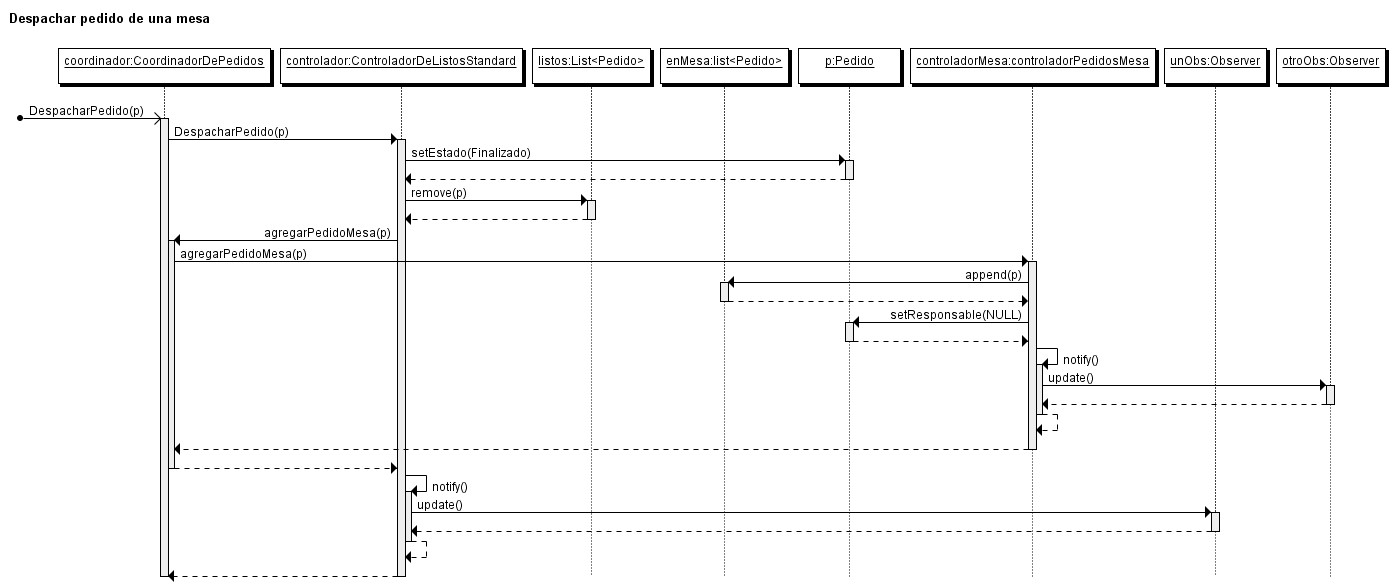
\includegraphics[height=5cm]{./figuras/despacharPedidoMesa.png}
\caption{Despacho de un pedido telefonico}
\end{figure}

Finalmente en el caso de un pedido de mostrador, el controlador de listos solo lo marca como terminado, ya que el pedido fue entregado y se conoce su forma de pago. Por lo tanto la secuencia es la siguiente:

\begin{figure}[H]
\centering
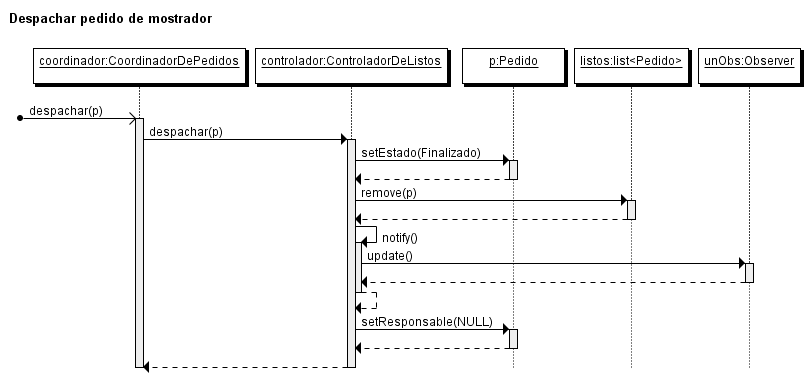
\includegraphics[height=5cm]{./figuras/despacharPedidoMostrador.png}
\caption{Despacho de un pedido telefonico}
\end{figure}

\subsubsection{Pedido de proximo pedido a preparar}
%TODO: decidir aridad de esta funci�n
%TODO: mostrar pseudocodigo

\subsubsection{Notificaci�n de entrega}

\subsubsection{Cerrado de mesa}

\subsubsection{Consulta de estado}

\section{Creaci�n y registro de pedidos}
En este componente se agrupan las clases que entran en juego al momento de crear un nuevo pedido.

La clase GeneradorDePedidos sirve de punto de entrada a este componente. El mismo posee el m�todo generarPedido, que es invocado por el Coordinador de pedidos, a fin de que se ingrese al sistema un nuevo pedido.

El Generador se encarga de llamar al controladorDeStock para que verifique que el stock existente sea capaz de satisfacer al pedido. Ademas el generador realiza el decremento del stock, y se encarga de realizar el callback a la gui en caso de que un insumo quede por debajo de su stock critico. %TODO: callback como?
El controlador de stock no es una clase abstracta porque creemos que no es probable que cambie su funcionamiento, el cual es bastante concreo, es decir revisar los elementos necesarios para armar los productos propios de un pedido y decrementar el stock. 

Luego de que se regisr� el decremento de stock, el Generador se encarga de llamar al EstimadorDeTiempos. Esta clase es abstracta, ya que pensamos que como la pizzeria desea ir refinando estas estimaciones, es probable que la forma de estimar se modifique de forma periodica. Por lo tanto, decidimos aplicar el \textit{Strategy pattern} a fin de poder lograr varias estrategias de estimaci�n. La Estimaci�n desarrollada en \ref{modifEstim} es implementada por la clase EstimadorBasico.

\textcolor{Red}{TODO: interacciones de estas clases con la GUI}

\textcolor{Red}{TODO: explicacion de metodos importantes}
\subsection{Modelado de escenarios}
\textcolor{Red}{TODO: escenarios que muestren el comportamiento de estas clases en los fenomenos pedidos en el enunciado}

\textcolor{Red}{TODO: pseudocodigos que muestren algoritmos como por ej estimacion de tiempos}

\section{Gesti�n de clientes}
Este componente es el responsable de validar clientes, para realizar las operaciones que requieren que se valide al usuario antes de proceder, como por ejemplo, ingresar un nuevo pedido telefonico. Por otro lado, este componente permite realizar el registro de nuevos usuarios en el sistema.

Basicamente son dos clases las relacionadas con este componente, la clase Cliente que modela la informaci�n necesaria de cada cliente registrado, asi como tambi�n permite crear nuevos clientes. 

Luego tenemos la clase ControladorCliente que se encarga de interactuar con la gui, validando los clientes segun distintos atributos.

\textcolor{Red}{TODO: interacciones de estas clases con la GUI}

\textcolor{Red}{TODO: explicacion de metodos importantes}
\subsection{Modelado de escenarios}
\textcolor{Red}{TODO: escenarios que muestren el comportamiento de estas clases en los fenomenos pedidos en el enunciado}

\section{Cocina}
La cocina es el componente de mayor complejidad del sistema. Al igual que en el manejo de pedidos fuera de la cocina, tenemos una clase que sirve de punto de entrada y de controlador de flujo dentro de la cocina, derivando a los pedidos al despachador o controlador correspondiente. Esta clase es la que tiene contacto con el controlador de ingresos, de modo que todo pedido que quiere entrar en la cocina pasa por este coordinador. Cuando recibe un pedido, o pide un pedido, esta clase es la que decide quien debe hacerse cargo de recibir al pedido. Si consideramos el funcionamiento actual de la pizzer�a, donde los pedidos que llegan a la cocina son preparables y cocinables, al ingresar un pedido a la cocina, el coordinador lo va a enviar al despachador de preparacion y luego cuando este lo termine se lo enviar� al despachador de cocci�n. 

El despachador de preparaci�n es una clase abstracta que tiene por responsabilidad mantener la cola de pedidos que deben ser preparados, conocer que subpedidos se prepararon y notifiar cuando el pedido ya fue preparado. Decidimos que sea abstracta porque es factible considerar que hay diferentes formas de manejar que pedido de los que estan esperando debe preparse a continuaci�n. Ademas, la implementaci�n de estas funcionalidades va a estar acoplada fuertemente con los tipos de productos existentes y el manejo que se le de a los mismos. Por ejemplo, es razonable que como la pizzer�a solo maneja pizzas y empanadas, las cuales son preparadas por un unico maestro, el despachador divida a un pedido en solo estas dos partes, sin embargo si en el futuro se agregan ensaladas, el pedido tendria que ser dividio de otra manera. Entonces a fin de dar mayor extensibilidad decidimos hacer que esta clase sea abstracta. En particular el despachador que se comporta como lo mostrado en la especificaci�n es implementado por DespachadorDePreparaci�nEstandard. Esta clase que hereda del despachador de preparaci�n, sabe distribuir pizzas y empanadas a sendos preparadores.

Preparador es una interfaz que tiene como metodo principal preparar. La idea es que este metodo sea el que hable con la gui para mostrar que se debe preparar. Decidimos hacer una interfaz para esto, porque si bien en este momento se muestra todo el contenido del pedido (o subpedido a preparar), esta estraetgia podr�a cambiar, si por ejemplo se desea tener un contro de cada producto del pedido. Entonces nuestro preparador especializado que implementa esta interfaz funciona como lo planteamos en la especificaci�n.

La clase despachadorDeHorno es la responsable del manejo de las colas de ingreso a los hornos, aplicando la politica correspondiente. En principio habiamos considerado que era conveniente separar la aplicaci�n de la politica del mantenimiento de las colas, sin embargo dado que la aplicaci�n de la politica requiere de un acceso completo a las colas, nos pareci� acertado acoplar ambas funcionalidades. La clase es abstracta, siguiendo el \textit{strategy pattern} a fin de permitir que se implementen diferentes politicas de manera flexible.

La clase ControladorHorno es una abstraccion de los modulos del horno, esta clase permite poner algo en un modulo, asi como tambi�n sacar algo de un modulo, o conocer que es lo que hay en cada modulo. Cada controladorHorno posee ademas un fraccionador que sabe fraccionar un pedido en partes que entran en un modulo, contando para eso con un diccionario que dado un tipo de pedido pueda decidir cuantos productos de ese tipo entran en cada modulo.

\textcolor{Red}{TODO: interacciones de estas clases con la GUI}

\textcolor{Red}{TODO: explicacion de metodos importantes}
\subsection{Modelado de escenarios}
\textcolor{Red}{TODO: escenarios que muestren el comportamiento de estas clases en los fenomenos pedidos en el enunciado}

\textcolor{Red}{TODO: pseudocodigos que muestren algoritmos como por ej seleccion de proximo pedido a cocinar}

\section{Gesti�n de stock y productos}
Como dijimos anteriormente, este componente es el que brinda las funcionalidades de ABM de stock y productos, asi como tambi�n permite acceder a la informaci�n sobre los diversos insumos y productos.

Sus clases principales son basicamente la clase Insumo y la clase Producto. 

Para realizar los ABM se decidio que la GUI utilice directamente los metodos de las clases antes nombradas, de modo que para crear un Insumo, lo que hace es invocar el new de Insumo, consideramos que esto si bien acopla un poco la GUI al sistema, creemos que no era necesario hacer un \textit{proxy} entre la GUI y estas clases, ya que la interacci�n era simple.

Otra clase propia de este componente es el Tipo de producto, que permite identificar por ejemplo a las pizzas, a las empanadas, asi como tambi�n, decir si un tipo de producto es cocinable, y$/$o preparable.
\textcolor{Red}{TODO: interacciones de estas clases con la GUI}


\subsection{Modelado de escenarios}
\textcolor{Red}{TODO: escenarios que muestren el comportamiento de estas clases en los fenomenos pedidos en el enunciado}

\textcolor{Red}{TODO: explicacion de metodos importantes}

\section{Cancelaci�n}
La cancelaci�n es un evento que involucra tanto al componente cocina como al componente de pedidos fuera de la cocina, por lo que podria incluso considerarse un componente separado. 

Mediante la interfaz grafica se selecciona un pedido y se invoca el metodo cancelar que posee el mismo, este metodo lo que hace es invocar el cancelar del responsable de cancelacion del pedido. Decidimos hacerlo de esta manera, en primer lugar, porque la cancelaci�n es un proceso que puede ser complejo, ya que por ejemplo, al cancelar un pedido que estaba en el horno, hay que avisar al maestro de que saque ese pedido, porque no hay que seguir cocinando. Sacar este pedido de la cocina puede implicar seleccionar un nuevo pedido a cocinar segun la politica vigente. De manera similar, una cancelaci�n de un pedido que se esta preparando requiere avisar al maestro de la cancelaci�n, para pedirle el stock reutilizable, asi como tambi�n buscar un nuevo pedido a preparar. Por esta raz�n, nos parece acertado que aquellos que pueden llegar a tener que efectuar acciones particulares debido a una cancelaci�n, sean invocados por el pedido cuando es cancelado. Notemos que este acercamiento es considerablemente extensible, ya que si se pretende por ejemplo agregar un nuevo controlador, solo debe implementar el m�todo cancelar y asegurarse de que aquellos pedidos que quedan bajo su control lo tienen a el como responsable de cancelarlo.

Ademas de esta manera de resolver el problema consideramos otras formas que no fueron aplicadas. En primer lugar, pensamos en que el pedido de cancelaci�n ingresar por el coordinador de pedidos, el cual va propagando el llamado a todos los agentes a los que tiene acceso, para que estos se fijen si les corresponde cancelar o no. Esto tiene como principal problema que se realiza un cantidad de llamadas innecesarias, pero como caracteristica positiva tiene que es bastante distribuida, ya que si bien el llamado entra por el coordinador, las invocaciones a cancelar se propagan a todos los posibles agentes.

Otra alternativa era considerar una clase canceladora que se encargue de rastrear el pedido, y luego decirle al controlador que lo estaba manejando en ese momento que lo cancele. El problema de esto es que el cancelador para buscar al responsable, va a tener que utilizar por ejemplo que los pedidos en tal estado si son de tal tipo estan bajo la orbita de tal controlador. Esto no nos parecio correcto, ni extensible, por lo cual se descart�.

Veamos a continuaci�n algunos escenarios diferentes de cancelaci�n.

El primer escenario consiste en cancelar un pedido que estaba en la cola de ingreso. En este caso se debe sacar de dicha cola al pedido y se debe reestablecer el stock de los insumos que no se van a utilizar.
%FIXME: como hacemos para subir el stock?
%TODO: diagramas de secuencia

En segundo lugar podemos considerar que ocurre cuando se cancela un pedido que esta en preparaci�n. En este caso puede ocurrir que el pedido se estaba preparando en el momento de su cancelaci�n, por lo que debe indicarse que se detenga la preparaci�n y que se indiquen que insumos se pueden salvar.
Veremos entonces que ocurre en estos casos, mostran en el primer escenario como se cancela un pedido de solo empanadas que estaba siendo preparado, suponiendo que luego se puede empezar a preparar otro pedido que estaba en espera.
Luego modelaremos el escenario en el que se cancela un pedido que ten�a su subpedido de pizzas preparado y su subpedido de empanadas sin preparar.
%FIXME: como hacemos para subir el stock?
%TODO: diagramas de secuencia

Otros lugar donde la cancelaci�n es mas conflictiva es durante la coccion de un pedido, si el mismo estaba en la cola el proceso es simple porque solo hay que sacarlo de la misma. Ahora si el pedido estaba en el horno o estaba a medio cocinar hay que avisar al maestro para que deje de cocinar el pedido.

Finalmente la cancelaci�n tambi�n puede darse en el ambito del controlador de entregas y del controlador de listos, en estos casos el manejo es simple, sin embargo, por ejemplo en el controlador de entregas, si la operatoria no fuera de contingencia podria requerir de una logica mas compleja de aviso al delivery.
%FIXME: entonces deberia ser una clase abstracta
\section{Clase Pedido}
\textcolor{Red}{TODO: explicacion de la clase pedido y las clases que lo heredan}

\section{Diagrama de clases}
\begin{landscape}
\begin{figure}[H]
\centering
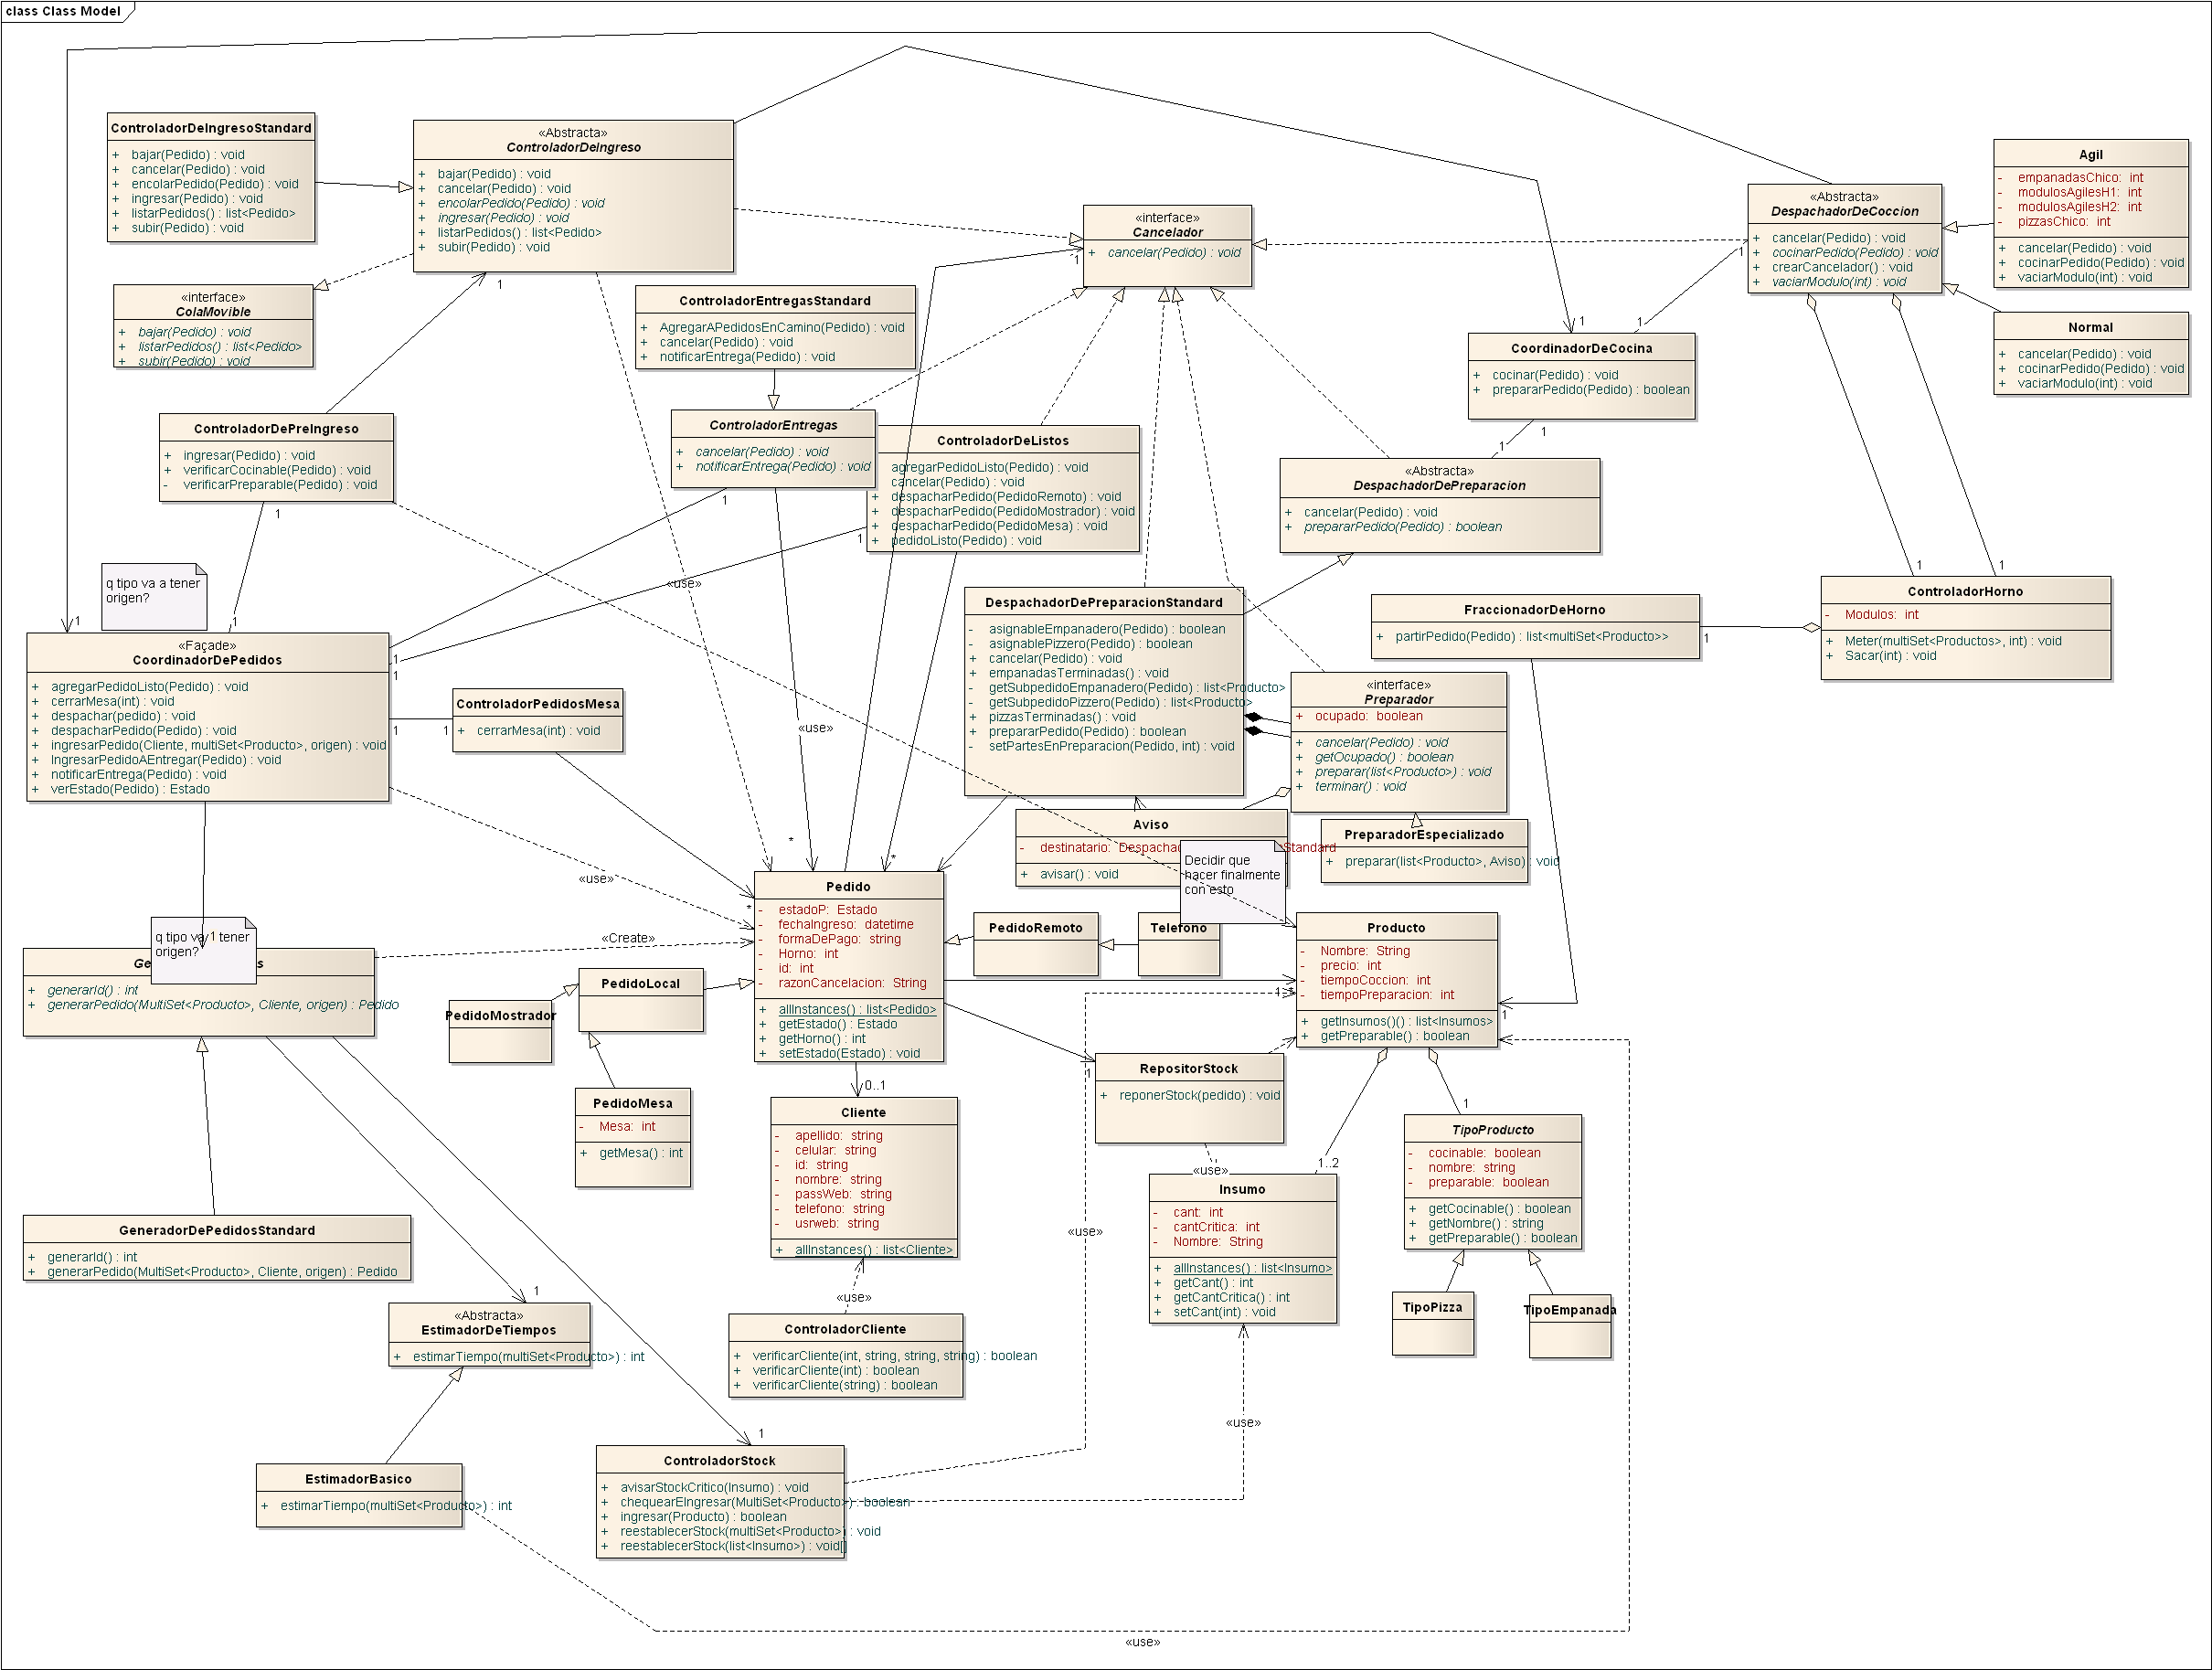
\includegraphics[height=18cm]{./figuras/clases.png}
\end{figure}
\end{landscape}
%
%\section{Explicaci�n de las clases}
%\clase
%{ABMproductos}
%{Esta clase se encarga de realizar las altas, bajas y modificaciones de los productos}
%{}{}
%
%\clase
%{ABMstock}
%{Esta clase se encarga de realizar las altas, bajas y modificaciones de los insumos}
%{}{}
%
%\clase
%{Agil}
%{Especializaci�n de gestor de horno, permite aplicar la politica agil}
%{}{}
%
%\clase
%{Aviso}
%{Clase utilizada para realizar el \textit{callback} desde el gestor de horno hacia el despachador de preparaci�n, es la encargada de ejecutar el metodo del despachador que lo notifica de que se termino de preparar algo. Esta clase permite que el despachador no necesite saber quien le avisa, y por lo tanto permite que los preparadores no requieran de metodos diferenciados para avisar que se terminaron de preparar las pizzas, o las empanadas}
%{}{}
%
%\clase{Cliente}
%{Esta clase representa a un cliente, conteniendo todos los datos del mismo.}
%{}{}
%
%\clase{ColaListos} %FIXME: nombre poco feliz
%{Esta clase contiene a los pedidos que ya estan listos. Su responsabilidad es la de conocer a todos los que estan en este estado, a fin de que despachar un pedido se haga desde esta clase}
%{}{}
%
%\clase
%{ControladorDeIngreso}
%{Controla la cola de ingreso, la cual puede ser modificada por el encargado de pedidos. Cuando algun preparador queda libre, envia el proximo pedido a preparar}
%{}{}
%
%\clase
%{ControladorCliente}
%{El controlador de cliente tiene por responsabilidad encargarse de autentificar un usuario}
%{}{}
%
%\clase
%{ControladorStock}
%{El controlador de stock, tiene por responsabilidad chequear la disponibilidad de insumos al momento de un ingreso, asi como la de hacer el decremento del stock al ingresar un pedido, generando el aviso de stock critico en caso de ser necesario.}
%{}{}
%
%\clase
%{CoordinadorDePedidos}
%{El coordinador de pedidos se encarga de controlar el ingreso de pedidos, y su ciclo de vida fuera de la cocina}
%{}{}
%
%\clase
%{DespachadorDePreparaci�n}
%{Esta clase tiene por responsabilidad manejar la cola de pedidos que se estan preparando, recordemos que puede existir una cola de preparaci'on si hay pedidos mixtos a la espera de uno de los maestros. El controlador de ingresos distribuye los pedidos a los distintos preparadores y despacha cada pedido a su gestor de horno correspondiente cuando ya esta preparado.}
%{}{}
%
%\clase
%{EstimadorDeTiempos}
%{El estimador de tiempos, como lo dice su nombre, se encarga de estimar el tiempo de preparacion y cocci�n de un pedido}
%{}{}
%
%\clase
%{GeneradorDePedidos}
%{Esta clase se encarga de crear pedidos, creando pedidos de solo bebidas o con comida segun los productos}%FIXME: justificacion
%{}{}
%
%\clase
%{GestorHorno}
%{Clase abstracta que permite implementar diferentes politicas para el manejo del horno}
%{}{}
%
%\clase
%{Insumo}
%{Contiene la informaci�n de los distintos insumos de la pizzer�a}
%{}{}
%
%\clase
%{Normal}
%{Permite implementar la politica normal de manejo del horno}
%{}{}
%
%\clase
%{Pedido}
%{Contiene la informaci�n de cada pedido}
%{}{}
%

\chapter{Modelado de escenarios}
A continuacion presentaremos diversos escenarios que permiten lograr un modelado del sistema basado en interacciones

\section{Ingreso de un pedido}
%TODO: escenario uno, ingresa un pedido de solo bebidas

%TODO: dos, ingresa un pedido de pizzas solamente y hay cosas en la cola de ingreso

%TODO: ingresa un pedido mixto y queda en la cola de listos, tener en cuenta q la seleccion de horno se hace mientras es intentna ingresar

\section{aviso de stock critico}

%TODO: no hay suficiente relleno de una empanada y de una pizza

\section{modificacion de la cola de pedidos}

%TODO: mover un pedido un lugar hacia arriba y otro hacia abajo

\section{Preparacion de pedidos}

%TODO: ingresa un pedido y no hay nada esperando preparandose tonces pasa a preparse

%TODO: se empieza a preparar un pedido mixto de la cola de ingreso

%TODO: maestro pide pedido a preparar y se le da un pedido que el otro maestro esta preparando

\section{Cocci�n de pedidos}

%TODO: se termina de prepara un pedido y no hay nada esperando

%TODO: se termina de prepara un pedido y se encola en su horno

%TODO: se termina de cocinar algo en un modulo agil y se toma un pedido chico

%TODO: se termina de cocinar algo en un modulo normal y se toma un pedido normal

%TODO: se termina de cocinar algo en un modulo y no hay nada a continuaci�n

%TODO: se saca un producto y se termino de cocinar

\section{Despachar pedido}

%TODO: se despacha un pedido remoto

%TODO: se despacha un pedido local

\section{Se cierra una mesa}

%TODO: se cierra una mesa y se registra la forma de pago

\section{Cancelacion}

%TODO: todos los escenarios de cancelacion

\section{Actualizar precios}

%TODO: modificar el precio de un pedido

\section{Consulta de estado de pedido}
El escenario a modelar es el siguiente: El encargado de pedidos abre la gui para consultar el estado de un pedido, entonces la gui muestra los pedidos y cuando el encargado encuentra el que busca, pide ver el estado. El coordinador es el encargado de hacer de adaptador entre la GUI y los pedidos.

En el diagrama suponemos que se llama un metodo de la gui verEstado, esto en verdad es abrir la interfaz para ver los estados de pedidos, es decir no es un metodo como tal, pero sirve para dar idea de que alguien le dice a la GUI que busque los pedidos y consulte el estado.

\begin{figure}[H]
\centering
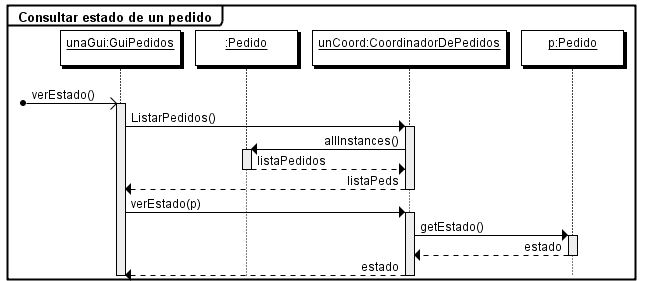
\includegraphics[scale=0.7]{./figuras/verEstado.png}
\end{figure}



\label{LastPage}
\end{document}
